\documentclass[a4paper,UTF8]{article}
\usepackage{ctex}
\usepackage[margin=1.25in]{geometry}
\usepackage{color}
\usepackage{graphicx}
\usepackage{amssymb}
\usepackage{amsmath}
\usepackage{amsthm}
\usepackage{enumerate}
\usepackage{bm}
\usepackage{hyperref}
\numberwithin{equation}{section}
%\usepackage[thmmarks, amsmath, thref]{ntheorem}
\theoremstyle{definition}
\newtheorem*{solution}{Solution}
\newtheorem*{prove}{Proof}
\newcommand{\indep}{\rotatebox[origin=c]{90}{$\models$}}

\usepackage{multirow}

%--

%--
\begin{document}
\title{机器学习导论\\
习题五}
\author{141242006, 袁帅, 141242006@smail.nju.edu.cn}
\maketitle
\section{[25pts] Bayes Optimal Classifier}
试证明在二分类问题中,但两类数据同先验、满足高斯分布且协方差相等时,LDA可产生贝叶斯最优分类器。
\begin{solution}
Suppose classes $c=\{1,2\}$, and the corresponding data distributions are $\mathcal{N}(\bm{\mu}_1, \bm{\Sigma})$ and $\mathcal{N}(\bm{\mu}_2, \bm{\Sigma})$. In Linear Discriminant Analysis(LDA), we find the vector $\bm{w}=\bm{S}_w^{-1}(\bm{\mu}_1-\bm{\mu}_2)$ to map data points on one single line. Since
\begin{equation}
\bm{S}_w=\sum_{\bm{x}\in X_1}(\bm{x}-\bm{\mu}_1)(\bm{x}-\bm{\mu}_1)^{\mathrm{T}}+\sum_{\bm{x}\in X_2}(\bm{x}-\bm{\mu}_2)(\bm{x}-\bm{\mu}_2)^{\mathrm{T}}=(m-2)\Sigma
\end{equation}
 is the unbiased estimation, we obtain $\bm{w}=\frac{1}{m-2}\Sigma^{-1}(\bm{\mu}_1-\bm{\mu}_2)$. Therefore, the prediction for $\bm{x}$ by LDA would be based on whether $\bm{w}^\mathrm{T}\bm{x}$ is closer to $\bm{w}^\mathrm{T}\bm{\mu}_1$ or $\bm{w}^\mathrm{T}\bm{\mu}_2$, which is equivalent to judge the sign of $\bm{w}^\mathrm{T}(\bm{x}-\frac{\bm{\mu}_1+\bm{\mu}_2}{2})$, so the resulting classifier would be
\begin{eqnarray}
\text{prediction}_{\text{LDA}}(\bm{x})=
\left\{
\begin{array}{ll}
1, &(\bm{\mu}_1-\bm{\mu}_2)^\mathrm{T}\Sigma^{-1}(\bm{x}-\frac{\bm{\mu}_1+\bm{\mu}_2}{2})>0,\\
2, &(\bm{\mu}_1-\bm{\mu}_2)^\mathrm{T}\Sigma^{-1}(\bm{x}-\frac{\bm{\mu}_1+\bm{\mu}_2}{2})<0.
\end{array}
\right.
\end{eqnarray}

Now, consider the Bayes Optimal Classifier: both classes have the same prior distribution, so by deciding whether $p(y=1|\bm{x})>p(y=2|\bm{x})$ or vice versa, we can focus on whether
\begin{eqnarray}
\frac{p(y=1|\bm{x})}{p(y=2|\bm{x})}&=&\frac{\frac{p(y=1)\cdot p(\bm{x}|y=1)}{p(\bm{x})}}{\frac{p(y=2)\cdot p(\bm{x}|y=2)}{p(\bm{x})}}=\frac{p(\bm{x}|y=1)}{p(\bm{x}|y=2)}=\frac{\frac{1}{(2\pi)^{d/2}|\Sigma|^{1/2}}\exp[-\frac{1}{2}(\bm{x}-\bm{\mu}_1)^\mathrm{T}\Sigma^{-1}(\bm{x}-\bm{\mu}_1)]}{\frac{1}{(2\pi)^{d/2}|\Sigma|^{1/2}}\exp[-\frac{1}{2}(\bm{x}-\bm{\mu}_2)^\mathrm{T}\Sigma^{-1}(\bm{x}-\bm{\mu}_2)]}\nonumber\\
&=&\exp[\frac{1}{2}(\bm{x}-\bm{\mu}_2)^\mathrm{T}\Sigma^{-1}(\bm{x}-\bm{\mu}_2)-\frac{1}{2}(\bm{x}-\bm{\mu}_1)^\mathrm{T}\Sigma^{-1}(\bm{x}-\bm{\mu}_1)]
\end{eqnarray}
is greater or less than 1. That is equivalent as whether
\begin{equation}
\frac{1}{2}[(\bm{x}-\bm{\mu}_2)^\mathrm{T}\Sigma^{-1}(\bm{x}-\bm{\mu}_2)-(\bm{x}-\bm{\mu}_1)^\mathrm{T}\Sigma^{-1}(\bm{x}-\bm{\mu}_1)]=(\bm{\mu}_1-\bm{\mu}_2)^\mathrm{T}\Sigma^{-1}(\bm{x}-\frac{\bm{\mu}_1+\bm{\mu}_2}{2})
\end{equation}
is positive or negative. Consequently, since both method's discriminant criteria are the same, LDA successfully generates a Bayes Optimal Classifier.
\end{solution}

\section{[25pts] Naive Bayes}
考虑下面的400个训练数据的数据统计情况,其中特征维度为2($\mathbf{x}=[x_1,x_2]$),每种特征取值0或1,类别标记$y\in\{-1,+1\}$。详细信息如表\ref{table:training}所示。

根据该数据统计情况,请分别利用直接查表的方式和朴素贝叶斯分类器给出$\mathbf{x}=[1,0]$的测试样本的类别预测,并写出具体的推导过程。
\begin{table}[h]
\centering
\caption{数据统计信息}
\label{table:training}\vspace{2mm}
\begin{tabular}{cc|cc}\hline
$x_1$		&  $x_2$ 	&	$y=+1$	&	$y=-1$ 	\\ \hline
0		&  0 	&	90	&	10 \\
0		&  1 	&	90 	&	10 \\
1		&  0 	&	51 	&	49 \\
1		&  1 	&	40 	&	60 \\\hline
\end{tabular}
\end{table}

\begin{solution}
According the table above, the prior distribution $P(y=+1)=\frac{90+90+51+40}{400}=0.6775$ and $P(y=-1)=\frac{10+10+49+60}{400}=0.3225$. The idea of Bayes classifier is to compute the posterior distribution $P(y|\bm{x})=\frac{P(y)P(\bm{x}|y)}{P(\bm{x})}$, and since the denominator $P(\bm{x})$ is identical to both classes, we obtain the discriminant criterion as
\begin{equation}
h(\bm{x})=\mathop{\arg\min}_{c\in\{+1,-1\}}P(y=c)P(\bm{x}|y=c)
\end{equation}

\paragraph{Bayes Optimal Classifier} If we directly refer to the table above, we find that more positive labels (51 vs. 49) are present in the $\bm{x}=[1,0]$ case. The result is equivalent as the Bayes Optimal Classifier.
The table indicates that the class-conditional distribution is given by $P(\bm{x}=[1,0]|y=+1)=\frac{51}{90+90+51+40}=0.1882$ and $P(\bm{x}=[1,0]|y=-1)=\frac{49}{10+10+49+60}=0.3798$, so we have
\begin{eqnarray}
P(y=+1)P(\bm{x}=[1,0]|y=+1)=0.6775\times 0.1882=0.1275,\\
P(y=-1)P(\bm{x}=[1,0]|y=-1)=0.3225\times 0.3798=0.1225.
\end{eqnarray}
The prediction for $\bm{x}=[1,0]$ would be +1.

\paragraph{Naïve Bayes Classifier} Naïve Bayes Classifiers assume attributes are conditionally independent, i.e. $P(\bm{x}=[1,0]|y=+1)=P(x_1=1|y=+1)P(x_2=0|y=+1)=\frac{51+40}{90+90+51+40}\cdot\frac{90+51}{90+90+51+40}=0.1747$, $P(\bm{x}=[1,0]|y=-1)=P(x_1=1|y=-1)P(x_2=0|y=-1)=\frac{49+60}{10+10+49+60}\cdot\frac{10+49}{10+10+49+60}=0.3865$. Therefore, 
\begin{eqnarray}
P(y=+1)P(\bm{x}=[1,0]|y=+1)=0.6775\times 0.1747=0.1184,\\
P(y=-1)P(\bm{x}=[1,0]|y=-1)=0.3225\times 0.3865=0.1246.
\end{eqnarray}
The prediction for $\bm{x}=[1,0]$ would be -1\footnote{If we do Laplacian correction, the result would be 0.1186 vs. 0.1244, which still yields a -1 prediction}.

\end{solution}

\section{\textbf{[25pts]} Bayesian Network}
贝叶斯网(Bayesian Network)是一种经典的概率图模型,请学习书本7.5节内容回答下面的问题:

(1) \textbf{[5pts]} 请画出下面的联合概率分布的分解式对应的贝叶斯网结构:
\begin{equation*}
P(A, B, C, D, E, F) = P(A)P(B)P(C)P(D|A)P(E|A)P(F|B, D)P(G|D, E)
\end{equation*}
\begin{figure}[h]
\label{3-1.pdf}
\centering
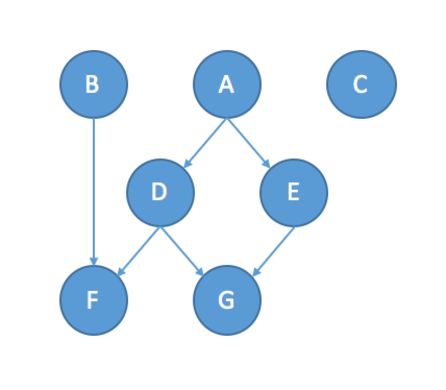
\includegraphics[scale=0.75]{3-1.pdf}
\caption{题目3-(1)有向图}
\end{figure}

(2) \textbf{[5pts]} 请写出图\ref{fig-DAG}中贝叶斯网结构的联合概率分布的分解表达式。
\begin{figure}[h]
\label{fig-DAG}
\centering
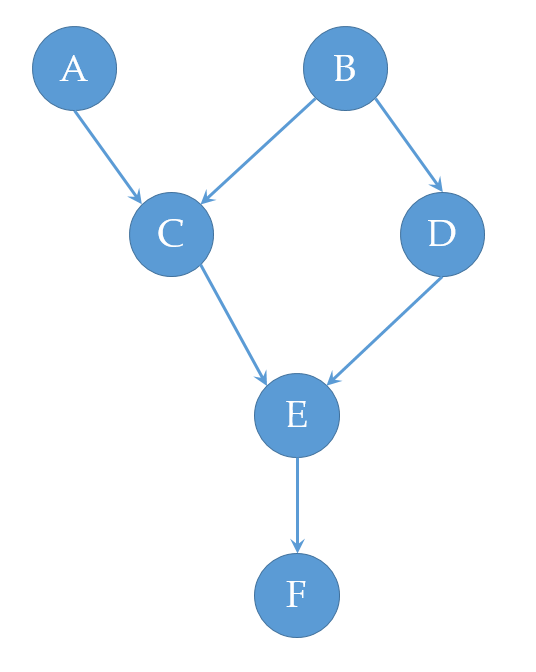
\includegraphics[scale=0.3]{bayes_net.png}
\caption{题目3-(2)有向图}
\end{figure}
\begin{equation*}
P(A, B, C, D, E, F) = P(A)P(B)P(C|A,B)P(D|B)P(E|C,D)P(F|E)
\end{equation*}

(3) \textbf{[15pts]} 基于第(2)问中的图\ref{fig-DAG}, 请判断表格\ref{table:DAG}中的论断是否正确,只需将下面的表格填完整即可。
\begin{table}[h]
\centering
\caption{判断表格中的论断是否正确}
\label{table:DAG}
\begin{tabular}{c|l|c||c|l|c}\hline
序号   		& 		关系  			& True/False 	& 序号   	& 		关系  			& True/False \\ \hline
1			&	$A \indep B$ 		    & 		True	    & 7  		& 	$F \indep B|C$ 		& 	False		 \\
2			&	$A \indep B|C$ 	    & 		False	    & 8  		& 	$F \indep B|C, D$ 	& 	True		 \\
3			&	$C \indep D $		    & 		False	    & 9  		& 	$F \indep B|E$ 		& 		True	 \\
4			&	$C \indep D|E$ 	    & 		False	    & 10  		& 	$A \indep F $			& 		False	 \\
5			&	$C \indep D|B, F$     & 		False	    & 11  		& 	$A \indep F|C$ 		& 	False		 \\
6			&	$F \indep B $		    & 		False	    & 12  		& 	$A \indep F|D$ 		& 	False		 \\ \hline
\end{tabular}
\end{table}
~\\

\section{[25pts] Naive Bayes in Practice}
请实现朴素贝叶斯分类器,同时支持离散属性和连续属性。详细编程题指南请参见链接:\url{http://lamda.nju.edu.cn/ml2017/PS5/ML5_programming.html}. 

同时,请简要谈谈你的感想。实践过程中遇到了什么问题,你是如何解决的?
\begin{solution}
The training process is just computing various distributions(prior, class-conditional, etc.), so no random factors are introduced. In training the model, numerical issues are fatal: the product of probabilities would vanish; the standard deviation could be zero, making Gaussian distribution doesn't work. Therefore, we take logarithms and add a small portion ($\epsilon\cdot \max(\sigma)$, $\epsilon=0.001$) to all $\sigma$. 

Since I did vectorization in MATLAB coding, the program terminates in \textbf{0.5 second} (training + predicting) on my MacBook Pro. The consequent accuracy is about \textbf{68.85\%}. 
~\\
\end{solution}
\end{document}